\section{BGP Wedgies and IP}
\subsection{Multiple Stable Configurations BGP Wedgies [RFC 4264]}
\begin{itemize}[nosep]
    \item Typical Policy
          \begin{itemize}[nosep]
              \item Prefer routes from customers
              \item Then prefer shortest paths
          \end{itemize}
\end{itemize}
\begin{figure}[H]
    \tikzsetnextfilename{bgp-wedgie-1}
    \begin{tikzpicture}[every node/.style={ellipse, fill=gray!40, minimum height=1cm, minimum width=1.5cm}, node distance=1cm]
        \node (1) {1};
        \node[above left=of 1,label=above left:{\textcolor{blue}{2 3 4 5 1}}] (2) {2};
        \node[above=of 2,label=above left:{\textcolor{blue}{3 4 5 1}}] (3) {3};
        \node[above right=of 1,label=above right:{\textcolor{blue}{5 1}}] (5) {5};
        \node[above =of 5,label=above right:{\textcolor{blue}{4 5 1}}] (4) {4};
        \draw (1) -- (2) node[pos=0.1,below left,fill=none,align=center] {1.2.0.0/16: 1 1 1 1\\(Backup Path)};
        \draw (2) -- (3);
        \draw (3) -- (4) node[pos=0.5,above,fill=none] {peering};
        \draw (4) -- (5);
        \draw (5) -- (1) node[pos=0.9,below right,fill=none,align=center] {1.2.0.0/16: 1\\Primary Path};;

        \path (5) -- (1) node[pos=0.5, draw,red,starburst,fill=orange,minimum height=2cm,minimum width=3cm,scale=0.25] {};

        \draw[red,thick,->] ([xshift=0.2cm]2.north) -- ([xshift=0.2cm]3.south);
        \draw[red,thick,->] ([yshift=-0.2cm]3.east) -- ([yshift=-0.2cm]4.west);
        \draw[red,thick,->] ([xshift=-0.2cm]4.south) -- ([xshift=-0.2cm]5.north);
        \draw[red,thick,->] (5.-155) -- (1.55);
    \end{tikzpicture}
\end{figure}

\begin{figure}[H]
    \tikzsetnextfilename{bgp-wedgie-2}
    \begin{tikzpicture}[every node/.style={ellipse, fill=gray!40, minimum height=1cm, minimum width=1.5cm}, node distance=1cm]
        \node (1) {1};
        \node[above left=of 1,label=above left:{\textcolor{blue}{2 1 1 1 1}}] (2) {2};
        \node[above=of 2,label=above left:{\textcolor{blue}{3 2 \dots}}] (3) {3};
        \node[above right=of 1,label=above right:{\textcolor{blue}{5 4 3 2 \dots}}] (5) {5};
        \node[above =of 5,label=above right:{\textcolor{blue}{4 3 2 \dots}}] (4) {4};
        \draw (1) -- (2) node[pos=0.1,below left,fill=none,align=center] {1.2.0.0/16: 1 1 1 1\\(Backup Path)};
        \draw (2) -- (3);
        \draw (3) -- (4) node[pos=0.5,above,fill=none] {peering};
        \draw (4) -- (5);
        \draw (5) -- (1) node[pos=0.9,below right,fill=none,align=center] {1.2.0.0/16: 1\\Primary Path};;

        \path (5) -- (1) node[pos=0.5, draw,red,starburst,fill=orange,minimum height=2cm,minimum width=3cm,scale=0.25] {};

        \draw[red,thick,->] ([xshift=0.2cm]3.south) -- ([xshift=0.2cm]2.north);
        \draw[red,thick,->] ([yshift=-0.2cm]4.west) -- ([yshift=-0.2cm]3.east);
        \draw[red,thick,->] ([xshift=-0.2cm]5.north) -- ([xshift=-0.2cm]4.south);
        \draw[red,thick,->] (2.-25) -- (1.125);
    \end{tikzpicture}
\end{figure}

\begin{figure}[H]
    \tikzsetnextfilename{bgp-wedgie-3}
    \begin{tikzpicture}[every node/.style={ellipse, fill=gray!40, minimum height=1cm, minimum width=1.5cm}, node distance=1cm]
        \node (1) {1};
        \node[above left=of 1,label=above left:{\textcolor{blue}{2 1 1 1 1}}] (2) {2};
        \node[above=of 2,label=above left:{\textcolor{blue}{3 2 \dots}}] (3) {3};
        \node[above right=of 1,label=above right:{\textcolor{blue}{5 1}}] (5) {5};
        \node[above =of 5,label=above right:{\textcolor{blue}{4 5 1}}] (4) {4};
        \draw (1) -- (2) node[pos=0.1,below left,fill=none,align=center] {1.2.0.0/16: 1 1 1 1\\(Backup Path)};
        \draw (2) -- (3);
        \draw (3) -- (4);
        \draw (4) -- (5);
        \draw (5) -- (1) node[pos=0.9,below right,fill=none,align=center] {1.2.0.0/16: 1\\Primary Path};;

        \draw[red,thick,->] ([xshift=-0.2cm]4.south) -- ([xshift=-0.2cm]5.north);
        \draw[red,thick,->] (5.-155) -- (1.55);
        \draw[red,thick,->] ([xshift=0.2cm]3.south) -- ([xshift=0.2cm]2.north);
        \draw[red,thick,->] (2.-25) -- (1.125);

        \node[red,above right=0.5cm and -2cm of 3,fill=none] {3 prefers customer route: stable configuration!};
    \end{tikzpicture}
\end{figure}

\subsection{BGP Security Goals}
\begin{itemize}[nosep]
    \item Confidential message exchange between neighbors
    \item \emph{Validity of routing information}
          \begin{itemize}[nosep]
              \item \emph{Origin, Path, Policy}
          \end{itemize}
    \item Correspondence to the data path
\end{itemize}

\subsection{Proposed Solution: S-BGP}
\begin{itemize}[nosep]
    \item Based on public key infrastructure
    \item Address attestations
          \begin{itemize}[nosep]
              \item Claims the right to originate a prefix
              \item Signed and distributed out of band
              \item Checked through delegation chain from ICANN
          \end{itemize}
    \item Route attestations
          \begin{itemize}[nosep]
              \item Attribute in BGP update message
              \item Signed by each AS as route along path
          \end{itemize}
    \item S-BGP can avoid
          \begin{itemize}[nosep]
              \item Prefix-hijacking
              \item Addition, removal, or reordering of intermediate ASes
          \end{itemize}
\end{itemize}

\subsection{S-BGP Deployment}
\begin{itemize}[nosep]
    \item Very challenging
          \begin{itemize}[nosep]
              \item PKI
              \item Accurate address registries
              \item Need to perform cryptographic operations on all path operations
              \item Flag day almost impossible
              \item Incremental deployment offers little incentive
          \end{itemize}
    \item But there is hope! [Goldberg et al, 2011]
          \begin{itemize}[nosep]
              \item Road to incremental deployment
              \item Change rules to break ties for secure paths
              \item If a few top tier-1 ISPs plus their respective stub clients
              \item deploy simplified version (just sign, not validate)
              \item Gains in traffic $\implies \$ \implies \text{adoption}$!
          \end{itemize}
\end{itemize}

\subsection{Data Plane Attacks}
\begin{itemize}[nosep]
    \item Routers/ASes can advertise one route, but not necessarily follow it!
    \item May drop packets
          \begin{itemize}[nosep]
              \item Or a fraction of packets
              \item What if you just slow down some traffic?
          \end{itemize}
    \item Can send packets in a different direction
          \begin{itemize}[nosep]
              \item Impersonation attack
              \item Snooping attack
          \end{itemize}
    \item How to detect?
          \begin{itemize}[nosep]
              \item Congestion or an attack?
              \item Can let ping/traceroute packets go through
              \item End-to-end checks?
          \end{itemize}
    \item Harder to pull off, as you need control of a router
\end{itemize}

\subsection{IP Protocol}
\begin{itemize}[nosep]
    \item Provides addressing and \emph{forwarding}
          \begin{itemize}[nosep]
              \item Addressing is a set of conventions for naming nodes in an IP network
              \item Forwarding is a local action by a router: passing a packet from input to output port
          \end{itemize}
    \item IP forwarding finds output port based on destination address
          \begin{itemize}[nosep]
              \item Also defines certain conventions on how to handle packets (e.g. fragmentation, time to live)
          \end{itemize}
    \item Contrast with \emph{routing}
          \begin{itemize}[nosep]
              \item Routing is the process of determining how to map packets to output ports (topic of next two lectures)
          \end{itemize}
\end{itemize}

\subsection{Service Model}
\begin{itemize}[nosep]
    \item Connectionless (datagram-based)
    \item Best-effort delivery (unreliable service)
          \begin{itemize}[nosep]
              \item packets may be lost
              \item packets may be delivered out of order
              \item duplicate copies of packets may be delivered
              \item packets may be delayed for a long time
          \end{itemize}
    \item It's the lowest common denominator
          \begin{itemize}[nosep]
              \item A network that delivers no packets fits the bill!
              \item All these can be dealt with above IP (if probability of delivery is non-zero\dots)
          \end{itemize}
\end{itemize}
\subsection{IPv4 Packet Format}
\begin{figure}[H]
    \begin{bytefield}{32}
        \bitheader{0-31}\\
        \bitboxes{4}{{Version}{IHL}} & \bitbox{8}{Type of Service} & \bitbox{16}{Total Length}\\
        \bitbox{16}{Identification} & \bitbox{3}{Flags} & \bitbox{13}{Fragment Offset}\\
        \bitboxes{8}{{Time to Live}{Protocol}} & \bitbox{16}{Header Checksum}\\
        \wordbox{1}{Source Address}\\
        \wordbox{1}{Destination Address}\\
        \bitbox{24}{Options} & \bitbox{8}{Padding}\\
        \wordbox[lr]{2}{data}\\
    \end{bytefield}
\end{figure}
\begin{figure}[H]
    \begin{bytefield}[bitwidth=\widthof{DF~}]{3}
        \bitheader{0-2}\\
        \begin{rightwordgroup}{Flags}
            \bitboxes{1}{0{DF}{MF}}
        \end{rightwordgroup}
    \end{bytefield}
\end{figure}

\subsection{IP Header Details}
\begin{itemize}[nosep]
    \item Forwarding based on destination address
    \item TTL (time-to-live) decremented at each hop
          \begin{itemize}[nosep]
              \item Originally was in seconds (no longer)
              \item Mostly prevents forwarding loops
              \item Other cool uses\dots
          \end{itemize}
    \item Fragmentation possible for large packets
          \begin{itemize}[nosep]
              \item Fragmented in network if crossing link with small frame
              \item MF: more fragments for this IP packet
              \item DF: don't fragment (returns error to sender)
          \end{itemize}
    \item Following IP header is ``payload'' data
          \begin{itemize}[nosep]
              \item Typically beginning with TCP or UDP header
          \end{itemize}
\end{itemize}

\subsection{Other fields}
\begin{itemize}[nosep]
    \item Version: 4 (IPv4) for most packets, there is also 6
    \item IHL: Internet Header Length: in 32-bit units (>5 implies options)
    \item Type of Service (won't go into this)
    \item Protocol Identifier (TCP: 6, UDP: 17, ICMP: 1, \dots)
    \item Checksum over the header
\end{itemize}

\subsection{Fragmentation and Reassembly}
\begin{itemize}[nosep]
    \item Each network has maximum transmission unit (MTU)
    \item Strategy
          \begin{itemize}[nosep]
              \item Fragment when necessary (MTU < size of datagram)
              \item Source tries to avoid fragmentation (why?)
              \item Re-fragmentation is possible
              \item Fragments are self-contained datagrams
              \item Delay reassembly until destination host
              \item No recovery of lost fragments
          \end{itemize}
\end{itemize}

\subsection{Fragmentation Example}
\begin{figure}[H]
    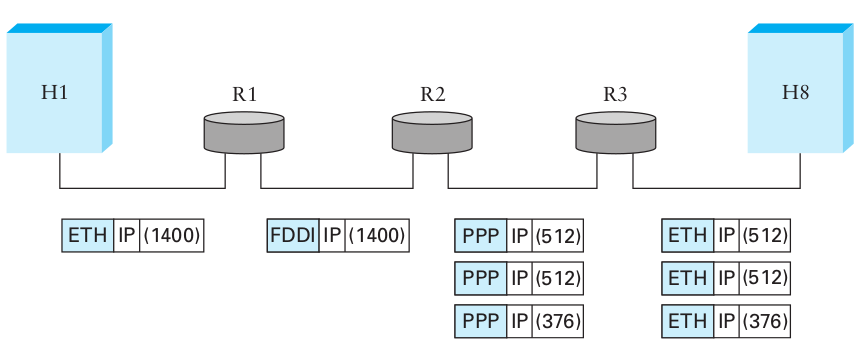
\includegraphics[scale=0.5]{lazy/fragmentationexample.png}
\end{figure}
\begin{itemize}[nosep]
    \item Ethernet MTU is 1,500 bytes
    \item PPP MTU is 576 bytes
          \begin{itemize}[nosep]
              \item R2 must fragment IP packets to forward them
          \end{itemize}
    \item IP addresses plus identification field identify fragments of same packet
    \item MF (more fragments bit) is 1 in all but last fragment
    \item Fragment offset multiple of 8 bytes
          \begin{itemize}[nosep]
              \item Multiply offset by 8 for fragment position original packet
          \end{itemize}
\end{itemize}

\subsection{Internet Control Message Protocol (ICMP)}
\begin{itemize}[nosep]
    \item Echo (ping)
    \item Redirect
    \item Destination unreachable (protocol, port, or host)
    \item TTL exceeded
    \item Checksum failed
    \item Reassembly failed
    \item Can't fragment
    \item Many ICMP messages include part of packet that triggered them
    \item see \url{https://www.iana.org/assignments/icmp-parameters/icmp-parameters.xhtml}
\end{itemize}

\subsection{ICMP message format}
\begin{figure}[H]
    \begin{bytefield}{32}
        \bitheader{0-31}\\
        \wordbox{2}{20-byte IP header\\(protocol=1-ICMP)}\\
        \bitboxes{8}{{Type}{Code}} & \bitbox{16}{Checksum}\\
        \wordbox[lr]{2}{Depend on type/code}
    \end{bytefield}
\end{figure}

\subsection{Example: Time Exceeded}
\begin{figure}[H]
    \begin{bytefield}{32}
        \bitheader{0-31}\\
        \wordbox{2}{20-byte IP header\\(protocol=1-ICMP)}\\
        \bitboxes{8}{{Type=11}{Code}} & \bitbox{16}{Checksum}\\
        \wordbox{1}{Unused}\\
        \wordbox{3}{IP header + first 8 payload bytes\\ of packet that caused ICMP to be generated}
    \end{bytefield}
\end{figure}

\subsection{Translating IP to lower level addresses}
\begin{itemize}[nosep]
    \item Map IP addresses into physical addresses
          \begin{itemize}[nosep]
              \item e.g. ethernet address of destination host
              \item or ethernet address of next hop router
          \end{itemize}
    \item Techniques
          \begin{itemize}[nosep]
              \item Encode physical address in host part of IP address (IPv6)
              \item Each network node maintains lookup table (IP$\to$physical)
          \end{itemize}
\end{itemize}

\subsection{ARP - \textit{address resolution protocol}}
\begin{itemize}[nosep]
    \item Dynamically builds table of IP to physical address bindings
    \item Broadcast request if IP address not in table
    \item All learn IP address of requesting node (broadcast)
    \item Target machine responds with its physical address
    \item Table entries are discarded if not refreshed
\end{itemize}

\subsection{ARP Ethernet frame format}
\begin{figure}[H]
    \begin{bytefield}[bitwidth=0.03\textwidth]{32}
        \bitheader{0,8,16,31}\\
        \bitboxes{16}{{$\texttt{Hardware Type} = 1$}{$\texttt{ProtocolType}=\texttt{0x0800}$}}\\
        \bitboxes{8}{{$\texttt{HLen} = 48$}{$\texttt{PLen} = 32$}} & \bitbox{16}{Operation}\\
        \wordbox{1}{\texttt{SourceHardwareAddr} (bytes 0 - 3)}\\
        \bitboxes{16}{{\texttt{SourceHardwareAddr} (bytes 4 - 5)}{\texttt{SourceProtocolAddr} (bytes 0 - 1)}}\\
        \bitboxes{16}{{\texttt{SourceProtocolAddr} (bytes 2 - 3)}{\texttt{TargetHardwareAddr} (bytes 0 - 1)}}\\
        \wordbox{1}{\texttt{TargetHardwareAddr} (bytes 2 - 5)}\\
        \wordbox{1}{\texttt{TargetProtocolAddr} (bytes 0 - 3)}
    \end{bytefield}
\end{figure}

\subsection{Format of IP Addresses}
\begin{itemize}[nosep]
    \item Globally unique (or made to seem that way)
          \begin{itemize}[nosep]
              \item 32-bit integers, read in groups of 8-bits: 128.148.32.110
          \end{itemize}
    \item Hierarchical: network + host
    \item Originally, a routing prefix embedded in address
          \begin{figure}[H]
              \begin{bytefield}{32}
                  \bitheader{0,1,7,8,31}\\
                  \bitbox{1}{0} & \bitbox{7}{Network} & \bitbox{24}{Host}
              \end{bytefield}
          \end{figure}
          \begin{figure}[H]
              \begin{bytefield}{32}
                  \bitheader{0,1,2,15,16,31}\\
                  \bitboxes{1}{10} & \bitbox{14}{Network} & \bitbox{16}{Host}
              \end{bytefield}
          \end{figure}
          \begin{figure}[H]
              \begin{bytefield}{32}
                  \bitheader{0,1,2,3,23,24,31}\\
                  \bitboxes{1}{110} & \bitbox{21}{Network} & \bitbox{8}{Host}
              \end{bytefield}
          \end{figure}
          \begin{itemize}[nosep]
              \item Class A (8-bit prefix), B (16-bit), C (24-bit)
              \item Routers need only know route for each network
          \end{itemize}
\end{itemize}

\subsection{Forwarding Tables}
\begin{itemize}[nosep]
    \item Exploit hierarchical structure of addresses: need to know how to reach \emph{networks}, not hosts
          \begin{table}[H]
              \begin{tabular}{l l}
                  Network     & Next Address \\\toprule
                  212.31.32.* & 0.0.0.0      \\
                  18.*.*.*    & 212.31.32.5  \\
                  128.148.*.* & 212.31.32.4  \\
                  Default     & 212.31.32.1  \\\bottomrule
              \end{tabular}
          \end{table}
    \item Keyed by network portion, not entire address
    \item Next address should be local
\end{itemize}

\subsection{Classed Addresses}
\begin{itemize}[nosep]
    \item Hierarchical: network + host
          \begin{itemize}[nosep]
              \item Saves memory in backbone routers (no default routers)
              \item Originally, routing prefix embedded in address
              \item Routers in same network must share network part
          \end{itemize}
    \item Inefficient use of address space
          \begin{itemize}[nosep]
              \item Class C with 2 hosts ($\sfrac{2}{255} = 0.78\%$ efficient)
              \item Class B with 256 hosts ($\sfrac{256}{65535} = 0.39\%$ efficient)
              \item Shortage of IP addresses
              \item Makes address authorities reluctant to give out class B's
          \end{itemize}
    \item Still too many networks
          \begin{itemize}[nosep]
              \item Routing table does not scale
          \end{itemize}
    \item Routing protocols do not scale
\end{itemize}

\subsection{Subnetting}
\begin{figure}[H]
    \begin{bytefield}{32}
        \bitboxes{16}{{Network Number}{Host Number}}\\
        \wordbox[]{1}{Class B Address}\\
        \bitbox{24}{111111111111111111111111} & \bitbox{8}{00000000}\\
        \wordbox[]{1}{Subnet Mask (255.255.255.0)}\\
        \bitbox{16}{Network Number} & \bitboxes{8}{{Subnet ID}{Host ID}}\\
        \wordbox[]{1}{Subnetted Address}
    \end{bytefield}
\end{figure}
\begin{itemize}[nosep]
    \item Add another level to address/routing hierarchy
    \item \emph{Subnet mask} defines variable portion of host part
    \item Subnets visible only within site
    \item Better use of address space
\end{itemize}

\subsection{Supernetting}
\begin{itemize}[nosep]
    \item Assign blocks of contiguous networks to nearby networks
    \item Called CIDR: Classless Inter-Domain Routing
    \item Represent blocks with a single pair
          \begin{itemize}[nosep]
              \item (first network address, count)
          \end{itemize}
    \item Restrict block sizes to powers of 2
    \item Use a bit mask (CIDR mask) to identify block size
    \item Address aggregation: reduce routing tables
\end{itemize}

\subsection{CIDR Forwarding Table}
\begin{table}[H]
    \begin{tabular}{ll}
        Network               & Next Address \\\toprule
        212.31.32/24          & 0.0.0.0      \\
        18/18                 & 212.31.32.5  \\
        128.148/16            & 212.31.32.4  \\
        \emph{128.148.128/17} & 212.31.32.8  \\
        0/0                   & 212.31.32.1
    \end{tabular}
\end{table}

\subsection{Obtaining IP Addresses}
\begin{itemize}[nosep]
    \item Blocks of IP addresses allocated hierarchically
          \begin{itemize}[nosep]
              \item ISP obtains an address block, may subdivide
                    \begin{table}[H]
                        \begin{tabular}{lll}
                                     & IP           & Binary                                          \\\toprule
                            ISP      & 128.35.16/20 & \underline{10000000 00100011 0001}0000 00000000 \\
                            Client 1 & 128.35.16/22 & \underline{10000000 00100011 000100}00 00000000 \\
                            Client 2 & 128.35.20/22 & \underline{10000000 00100011 000101}00 00000000 \\
                            Client 3 & 128.35.24/21 & \underline{10000000 00100011 000110}00 00000000 \\
                        \end{tabular}
                    \end{table}
          \end{itemize}
    \item Global allocation: ICANN, /8's (\emph{ran out!})
    \item Regional registries: ARIN, RIPE, APNIC, LACNIC, AFRINIC
\end{itemize}